\newpage
\section{Casi d'uso}
testo

	\subsection{Introduzione}
	testo
	
	\subsection{Attori}
	\begin{itemize}
		\item Producer
		\item Utente che interagisce con il gestore personale
		\item Consumer (secondario)
	\end{itemize}
	
	\subsection{Elenco casi d'uso}
	Messaggio - tecnologia che invia il messaggio - tipo di messaggio di quella tecnologia.
	Classificazioni in base al topic.


%TODO: da ricordarsi: se qualcuno è offline, c'è la possibilità che il messaggio venga perso.



\subsubsection{UC1 - Redmine/GitLab genera una segnalazione}
	\begin{itemize}
		\item \textbf{Codice}: UC1.
		\item \textbf{Titolo}: Redmine/GitLab genera una segnalazione.
		\item \textbf{Attori primari}: Redmine/Gitlab.
		\item \textbf{Descrizione}:
		 il sistema qui è il Producer ed è interno al sistema Butterfly. Cambio stato repository tramite commit per GitLab. Cambio di stato issue tracking system per GitLab e Redmine.
		\item \textbf{Precondizione}: c'è qualcosa da segnalare
		\item \textbf{Postcondizione}: segnalazione generata e inviata
		\item \textbf{Scenario principale}: 
		\begin{enumerate}
			\item Redmine/GitLab prepara una segnalazione da mandare
			\item Redmine/GitLab invia la segnalazione al Producer.
		\end{enumerate}
		
	\end{itemize}

\subsubsection{UC1.1 - Redmine/GitLab crea e invia un messaggio per il Producer}
	\begin{itemize}
		\item \textbf{Codice}: UC1.1.
		\item \textbf{Titolo}: Redmine/GitLab crea e invia un messaggio per il Producer.
		\item \textbf{Attori primari}: Redmine/Gitlab.
		\item \textbf{Descrizione}:
		il sistema qui è il Producer ed è interno al sistema Butterfly. Cambio stato repository tramite commit per GitLab. Cambio di stato issue tracking system per GitLab e Redmine.
		\item \textbf{Precondizione}: 
		\item \textbf{Postcondizione}: segnalazione generata e inviata al Producer
		\item \textbf{Scenario principale}: 
		\begin{enumerate}
			\item Redmine/GitLab prepara una segnalazione da mandare
			\item Redmine/GitLab invia la segnalazione al Producer.
		\end{enumerate}
		\item \textbf{Estensioni}: messaggio creato con parametri errati.
	\end{itemize}
	

\subsubsection{UC1.2 - Redmine/GitLab genera una segnalazione errata}
	\begin{itemize}
		\item \textbf{Codice}: UC1.2.
		\item \textbf{Titolo}: Redmine/GitLab genera una segnalazione errata.
		\item \textbf{Attori primari}: Redmine/Gitlab.
		\item \textbf{Descrizione}:
		\item \textbf{Precondizione}:
		\item \textbf{Postcondizione}: non viene inviato a Producer
		\item \textbf{Scenario principale}: 
	\end{itemize}

\subsubsection{UC2 - Il Producer invia la segnalazione al Broker}
	\begin{itemize}
		\item \textbf{Codice}: UC2.
		\item \textbf{Titolo}: il Producer invia la segnalazione al Broker.
		\item \textbf{Attori primari}: Producer.
		\item \textbf{Descrizione}: ..il sistema qui è Broker ed è interno al sistema Butterfly.
		\item \textbf{Precondizione}:
		\item \textbf{Postcondizione}:
		\item \textbf{Scenario principale}: 
	\end{itemize}

%Opzionale Sonarqube

\subsubsection{UC3 - Il Consumer interroga il Broker}
	\begin{itemize}
		\item \textbf{Codice}: UC3.
		\item \textbf{Titolo}: il Consumer interroga il Broker.
		\item \textbf{Attori primari}: Consumer.
		\item \textbf{Descrizione}: il Consumer chiede al Broker per acquisire il messaggio... il sistema di riferimento qui è Broker ed è interno al sistema Butterfly.
		\item \textbf{Precondizione}:
		\item \textbf{Postcondizione}:
		\item \textbf{Scenario principale}: 
	\end{itemize}


\subsubsection{UC4 - Telegram/mail riceve un messaggio dal Consumer} 
	\begin{itemize}
		\item \textbf{Codice}: UC4.
		\item \textbf{Titolo}: Telegram/mail riceve un messaggio dal Consumer.
		\item \textbf{Attori}: Telegram/server mail.
		\item \textbf{Descrizione}: il sistema di riferimento qui è il Consumer ed è interno al sistema Butterfly.
		Sebbene questo caso d'uso non sia del tutto corretto perchè l'attore Telegram/mail è un attore passivo, che riceve e non che agisce, è stato scelto di creare questo caso d'uso al fine di inserire la funzionalità "Il Consumer invia un messaggio a Telegram/mail". Ma scrivere un caso d'uso in tal modo sarebbe stato del tutto scorretto in quanto il sistema di riferimento in questo caso sarebbe stato Telegram/mail. Cosa non possibile dato che Telegram/mail è esterno a Butterfly e quindi non può essere considerato un suo sottosistema.
		\item \textbf{Precondizione}: il Consumer invia un messaggio a Telegram/server email in seguito a un'interrogazione del broker.
		\item \textbf{Postcondizione}: Telegram/server mail riceve il messaggio
		\item \textbf{Scenario principale}:
		\begin{enumerate}
			\item La ricezione del messaggio va a buon fine
		\end{enumerate} 
	\end{itemize}

%Opzionale Slack


\subsubsection{UC5 - Accesso}
		\begin{figure}[H]
			\centering
				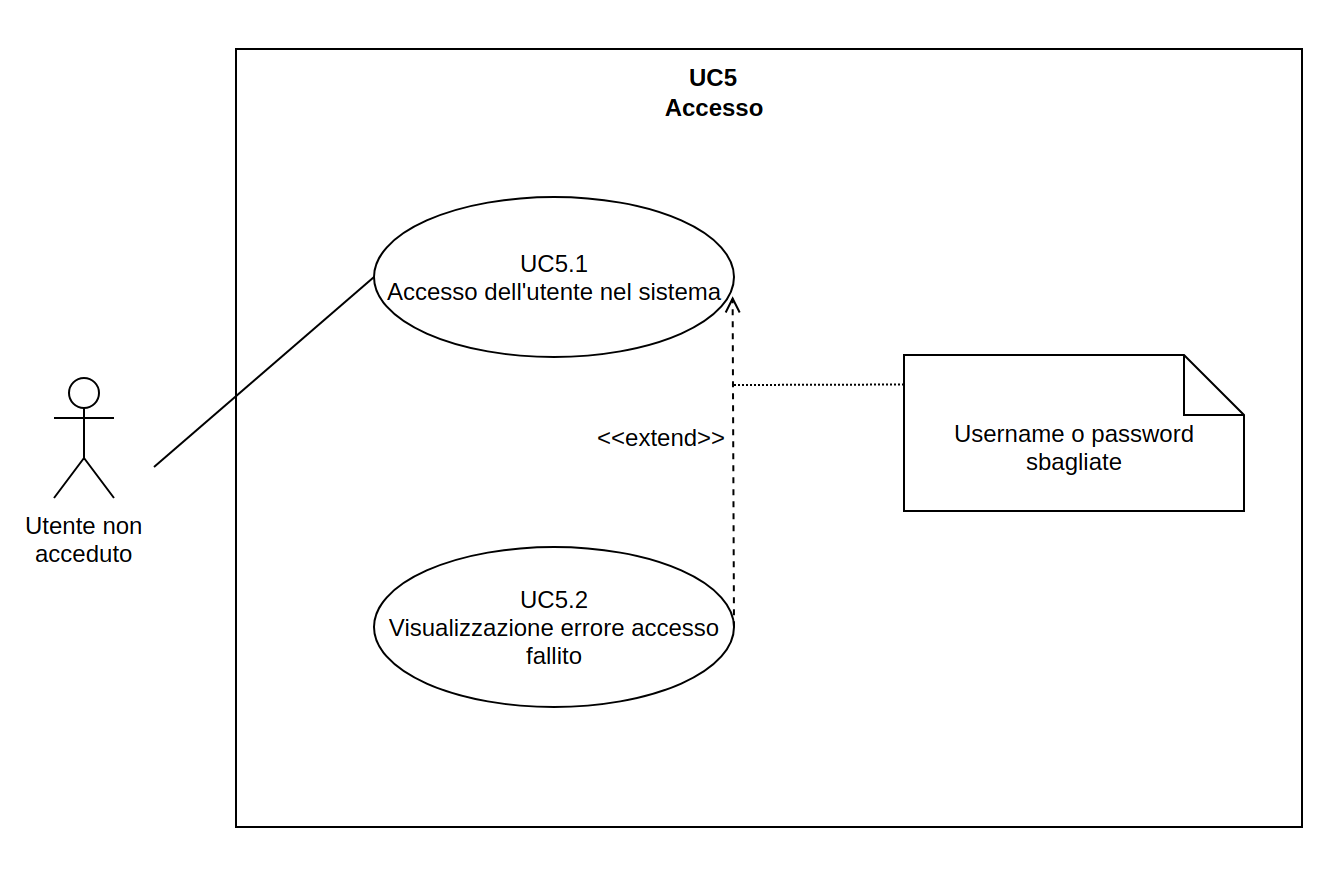
\includegraphics[width=\columnwidth]{img/UC5.png}\\
			\caption{UC5 - Accesso}
		\end{figure}
	\begin{itemize}
		\item \textbf{Codice}: UC5
		\item \textbf{Titolo}: accesso
		\item \textbf{Attori primari}: utente non acceduto
		\item \textbf{Descrizione}: l'utente richiede di accedere al sistema attraverso un form dove inserisce username e password
		\item \textbf{Precondizione}: il sistema considera l’utilizzatore come un utente non acceduto
		\item \textbf{Postcondizione}: il sistema riconosce l'utilizzatore come utente acceduto
		\item \textbf{Scenario Principale}: l'utente non ancora riconosciuto dal sistema effettua l'accesso.
	\end{itemize}
	
	\paragraph{UC5.1 - Accesso dell'utente nel sistema}
		\begin{figure}[H]
			\centering
				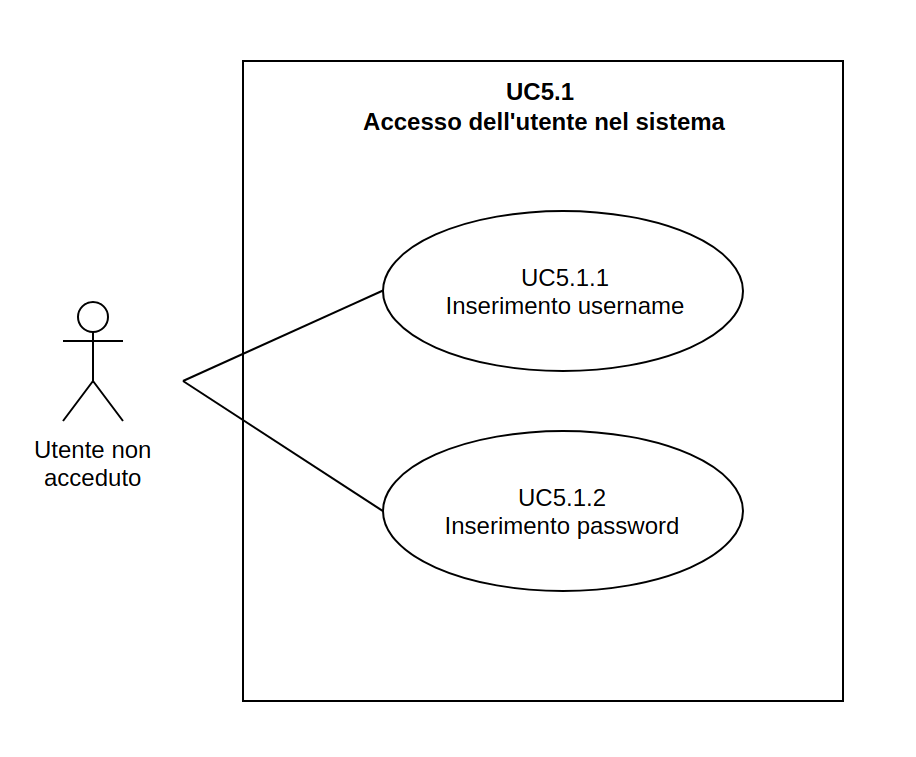
\includegraphics[width=\columnwidth]{img/UC5_1.png}\\
			\caption{UC5.1 - Accesso dell'utente nel sistema}
		\end{figure}
		\begin{itemize}
			\item \textbf{Codice}: UC5.1
			\item \textbf{Titolo}: accesso dell'utente nel sistema
			\item \textbf{Attori}: utente non acceduto
			\item \textbf{Descrizione}: l'utente attende l'autenticazione da parte del sistema
			\item \textbf{Precondizione}: il sistema riconosce l'utilizzatore come un utente non autenticato
			\item \textbf{Postcondizione}: il sistema riconosce l'utente autenticato con successo
			\item \textbf{Scenario Principale}: l’utente non ancora riconosciuto dal sistema richiede l'autenticazione
			\item \textbf{Estensioni}:
			\begin{enumerate}
				\item Nel caso in cui l'accesso non dovrebbe andare a buon fine viene visualizzato un errore avvisando l'utente [UC5.2].
			\end{enumerate}
	\end{itemize}

		\subparagraph{UC5.1.1 - Inserimento username}
			\begin{itemize}
				\item \textbf{Codice}: UC5.1.1
				\item \textbf{Titolo}: inserimento username
				\item \textbf{Attori}: utente non acceduto
				\item \textbf{Descrizione}: l'utente inserisce l'username
				\item \textbf{Precondizione}: il sistema offre l'interfaccia grafica adatta all'inserimento dell'username
				\item \textbf{Postcondizione}: l'utente ha inserito l'username desiderato
				\item \textbf{Scenario Principale}: l'utente inserisce l'username per autenticarsi.
			\end{itemize}
		
		\subparagraph{UC5.1.2 - Inserimento password}
			\begin{itemize}
				\item \textbf{Codice}: UC5.1.2	
				\item \textbf{Titolo}: inserimento password
				\item \textbf{Attori}: utente non acceduto
				\item \textbf{Descrizione}: l'utente inserisce la password
				\item \textbf{Precondizione}: il sistema offre l'interfaccia grafica adatta all'inserimento della password
				\item \textbf{Postcondizione}: l'utente ha inserito la password desiderata
				\item \textbf{Scenario Principale}: l'utente inserisce la password per autenticarsi.
			\end{itemize}
		
%Da aggiungere al limite più avanti
		
%		\subparagraph{UC5.1.2}
%			\begin{itemize}
%			\item \textbf{Codice}: UC6.1.2.
%			\item \textbf{Titolo}: inserimento password
%			\item \textbf{Attori}: utente non autenticato
%			\item \textbf{Descrizione}: l'utente inserisce la password
%			\item \textbf{Precondizione}: il sistema offre l'interfaccia grafica adatta all'inserimento della password
%			\item \textbf{Postcondizione}: l'utente ha inserito la password desiderata
%			\item \textbf{Scenario Principale}: l'utente inserisce la password per autenticarsi
%		\end{itemize}
	
	\paragraph{UC5.2 - Visualizzazione errore autenticazione fallita}
		\begin{itemize}
			\item \textbf{Titolo}: visualizzazione errore autenticazione fallita
			\item \textbf{Attori}: utente non autenticato
			\item \textbf{Descrizione}: l'utente viene avvisato che ha inserito username o password errate
			\item \textbf{Precondizione}: il sistema riceve una richiesta di accesso da parte di un utente che
			fornisce username o password sbagliate
			\item \textbf{Postcondizione}: il sistema comunica all'utilizzatore l'errore
			\item \textbf{Scenario Principale}: l'utente visualizza il messaggio d'errore.
		\end{itemize}



\subsubsection{UC6 - Modifica delle preferenze}
	\begin{itemize}
		\item \textbf{Codice}: UC6.
		\item \textbf{Titolo}: modifica delle preferenze.
		\item \textbf{Attori}: 
		\item \textbf{Descrizione}: modifica delle preferenze dell'utente nel sistema.
		\item \textbf{Precondizione}: 
		\item \textbf{Postcondizione}: 
		\item \textbf{Scenario Principale}:
	\end{itemize}



	\paragraph{UC6.1 - Aggiunta preferenze}
	\begin{itemize}
		\item \textbf{Codice}: UC6.1.
		\item \textbf{Titolo}: aggiunta preferenze.
		\item 
	\end{itemize}
	
	\subparagraph{UC6.1.1 - Iscrizione topic}
	\begin{itemize}
		\item \textbf{Codice}: UC6.1.1.
		\item \textbf{Titolo}: aggiunta preferenze.
		\item \textbf{Descrizione}: data la lista di topic presenti l'utente seleziona quelli a cui è interessato ricevere notifica (suddiviso per tecnologia e per tag [BUG, FIX, ISSUE, ecc.] ).
	\end{itemize}
		
			
	\subparagraph{UC6.1.2 - Aggiunta dei giorni di indisponibilità nel calendario} 
	\begin{itemize}
		\item \textbf{Codice}: UC6.1.2.
		\item \textbf{Titolo}: aggiunta dei giorni di indisponibilità nel calendario.
		\item \textbf{Descrizione}: dato il calendario lavorativo l'utente selezionerà i giorni in cui sarà assente.
	\end{itemize}
			
	\subparagraph{UC6.1.3 - Aggiunta della piattaforma di messaggistica}
	\begin{itemize}
		\item \textbf{Codice}: UC6.1.3.
		\item \textbf{Titolo}: aggiunta della piattaforma di messaggistica.
		\item \textbf{Descrizione}: 
		%telegram: nickname e mail sono già salvati nel DB
	\end{itemize}
			



	\paragraph{UC6.2 - Rimozione preferenza}
	\begin{itemize}
		\item \textbf{Codice}: UC6.2.
		\item \textbf{Titolo}: rimozione preferenza.
		\item \textbf{Descrizione}: 
	\end{itemize}
	
	
	\subparagraph{UC6.2.1 - Disiscrizione topic}
	\begin{itemize}
		\item \textbf{Codice}: UC6.2.1.
		\item \textbf{Titolo}: disiscrizione topic.
		\item \textbf{Descrizione}: data la lista di topic a cui è iscritto l'utente elimina quelli a cui non è più interessato ricevere notifica.
	\end{itemize}
	
			
	\subparagraph{UC6.2.2 - Rimozione giorno di indisponibilità nel calendario}
	\begin{itemize}
		\item \textbf{Codice}: UC6.2.2.
		\item \textbf{Titolo}: rimozione giorno di indisponibilità nel calendario.
		\item \textbf{Descrizione}: data una lista dei giorni in cui non si è reperibili, vengono rimossi uno o più di questi giorni.
	\end{itemize}
			
			
	\subparagraph{UC6.2.3 - Rimozione piattaforma di messaggistica}
	\begin{itemize}
		\item \textbf{Codice}: UC6.2.3.
		\item \textbf{Titolo}: rimozione piattaforma di messaggistica.
		\item \textbf{Descrizione}: 
	\end{itemize}

%Da tenere in considerazione per la pagina da creare più avanti	
%	\paragraph{UC7.4}
%	Annullo le modifiche fatte

		
